\chapter{Tabellenkalkulation}\label{ch:Lektion}
\begin{mycaution}
Dokumentation der wichtigsten Excel-Funktionen: \url{https://ict.mygymer.ch/tabellenkalkulation/}
\end{mycaution}
\section{Aufgaben}

\begin{mysubmission}[Datentypen und Sortierung]
Speichern Sie die Datei \texttt{himmelskoerper.xlsx} auf Ihrem Computer.

Öffnen Sie die Datei und wählen Sie die Tabelle \texttt{Asteroiden} aus.

Sie sollen nun die Tabelle nacheinander nach unterschiedlichen Kriterien sortieren. Nach jedem Sortieren ist die Reihenfolge der Zeilen anders, und Sie notieren sich den Anfangsbuchstaben des Asteroiden auf der angegebenen Zeile. Die Anfangsbuchstaben ergeben ein Lösungswort.

\textbf{Wichtig:} Die zusammengehörenden Werte pro Zeile müssen natürlich so bleiben, d.h. auf der Zeile des Asteroiden \texttt{Psyche} muss \textit{immer} sein Durchmesser \texttt{253} stehen.

\textbf{Achtung:} In der Spalte \texttt{C} hat ein Wert den falschen Datentyp, so dass die Sortierung nicht korrekt ist. Um das richtige Lösungswort zu erhalten, müssen Sie den Fehler vor dem Sortieren korrigieren.

\begin{table}[H]
    \centering
    \begin{tabular}{p{10cm}|l}
        \toprule
        Sortierung & Anfangsbuchstabe \\ 
        \midrule\midrule
        1. Mittlerer Durchmesser aufsteigend & Zeile 11 \\ 
        2. Namen des Asteroiden rückwärts (von Z bis A) & Zeile 13 \\ 
        3. Mittlere Entfernung zur Sonne aufsteigend & Zeile 6 \\ 
        4. Nachname des Entdeckers vorwärts (von A bis Z) \& mittlerer Durchmesser aufsteigend & Zeile 5 \\ 
        \bottomrule
    \end{tabular}
    \caption{Sortierungen und Anfangsbuchstaben}
\end{table}
Geben Sie das Lösungswort auf Moodle ab.
\begin{myanswer}
Bei Juno ist die mittlere Entfernung zur Sonne ein Wert vom Datentyp Text. Die Ursache ist, dass ein falsches Dezimaltrennzeichen verwendet worden ist (Komma statt Punkt).

\textbf{Achtung}: Je nach Ländereinstellung des Betriebssystems oder des Office-Pakets ist das Dezimaltrennzeichen unterschiedlich, in Deutschland ist es beispielsweise das Komma!

Das korrekte Lösungswort lautet ``\textbf{HEBE}'', das ist der Name eines weiteren Asteroiden.
\end{myanswer}
\end{mysubmission}


\begin{mychallenge}
Versuchen Sie, die Asteroiden nach dem Datum der Entdeckung zu sortieren. Warum funktioniert das nicht? Überlegen Sie sich, wie Sie das Datum darstellen könnten, damit das Sortieren wie gewünscht funktioniert.
\begin{myanswer}
Zusatzaufgabe: In Excel können Daten vor dem 1.1.1900 nicht als Zahlenwert eingegeben werden. Eine korrekte Sortierung kann so erreicht werden:

\begin{itemize}
\item  Eine Datumsdarstellung wählen, welche als Text korrekt sortiert wird, z.B. ``1892-02-25''.
\item Jahr, Monat und Tag als Zahl in separaten Spalten eingeben, danach die Sortierebenen Jahr, Monat und Tag wählen.
\item Mit LibreOffice arbeiten.
 \end{itemize}
\end{myanswer}
\end{mychallenge}

\begin{mysubmission}[Zahlenformate]
Verwenden Sie für diese Aufgabe die Datei aus der Aufgabe \texttt{Datentypen und Sortierung}.

Öffnen Sie das Tabellenblatt \texttt{Planeten}.

Formatieren Sie die Zellen wie folgt:
\begin{table}[H]
    \centering
    \begin{tabular}{p{7cm}|p{7cm}}
        \toprule
        \textbf{Zellinhalt} & \textbf{Formatierung} \\ 
        \midrule\midrule
        Grosse Bahnhalbachse (Spalte B) & Mit Tausendertrennzeichen ohne Dezimalstellen \\\midrule
        Numerische Exzentrizität der Bahn (Spalte C) & Drei Dezimalstellen \\\midrule
        Umlaufperiode (Spalte D) & Zwei Dezimalstellen \\\midrule
        Mittlerer Äquatorradius (Spalte E) & Eine Dezimalstelle und Tausendertrennzeichen \\\midrule
        Mittlerer Äquatorradius relativ zur Erde (Spalte F) & Als Prozent \\\midrule
        Volumen (Spalte G) & Als Exponentialzahl \\\midrule
        Masse (Spalte H) & Als Exponentialzahl mit vier Dezimalstellen \\
        \bottomrule
    \end{tabular}
\end{table}
Geben Sie einen Screenshot Ihres fertig formatierten Arbeitsblatts auf Moodle ab.

\begin{myanswer}
\begin{figure}[H]
\centering
\includegraphics[width=\linewidth]{"GrundlagenInfo/09_Tabellenkalkulation/Screenshots/loesung 1-3"}
\end{figure}
\end{myanswer}

\end{mysubmission}

\begin{mysubmission}[Diagramme]
Verwenden Sie für diese Aufgabe die Datei \texttt{diagramme.xlsx}.

\paragraph*{a) Schweizer Bevölkerung nach Nationalität}
Wählen Sie einen geeigneten Diagrammtyp, um die Daten darzustellen. Das Diagramm muss Folgendes enthalten:
\begin{itemize}
    \item aussagekräftiger Diagrammtitel
    \item Datenbeschriftungen
    \item Legende
\end{itemize}

\paragraph*{b) Frauenanteil im Nationalrat nach Parteien}
Wählen Sie einen geeigneten Diagrammtyp, um die Daten darzustellen. Das Diagramm muss Folgendes enthalten:
\begin{itemize}
    \item aussagekräftiger Diagrammtitel
    \item Achsentitel für die vertikale Achse
    \item Legende
\end{itemize}

\paragraph*{c) Zeitliche Entwicklung der Nationalratsmandate nach Parteien}
Wählen Sie einen geeigneten Diagrammtyp, um die Daten darzustellen. Das Diagramm muss wie folgt gestaltet sein:
\begin{itemize}
    \item aussagekräftiger Diagrammtitel
    \item Achsentitel für die vertikale Achse
    \item Legende
    \item Die horizontale Achse muss von 1931 bis 2015 reichen und muss in Intervalle von vier Jahren unterteilt sein.
\end{itemize}

\paragraph*{d) Entwicklung der Weltbevölkerung}
Im Tabellenblatt sind zwei Tabellen zur Entwicklung der Weltbevölkerung vorhanden. Erstellen Sie:
\begin{itemize}
    \item aus der linken Tabelle ein Liniendiagramm
    \item aus der rechten Tabelle ein Punktdiagramm.
\end{itemize}
Beide Diagramme sollen so gestaltet werden:
\begin{itemize}
    \item aussagekräftiger Diagrammtitel
    \item Achsentitel für beide Achsen
    \item Die horizontale Achse muss bei 0 beginnen und bei 2015 enden.
    \item Die vertikale Achse soll die Anzeigeeinheit \texttt{Millionen} haben.
\end{itemize}

Vergleichen Sie die beiden Diagramme.
\begin{itemize}
    \item Warum sehen die Diagramme unterschiedlich aus?
    \item Welches ist aussagekräftiger und warum?
\end{itemize}

Geben Sie Screenshots Ihrer fertig formatierten Diagramme auf Moodle ab.

\begin{myanswer}

\begin{figure}[H]
\centering
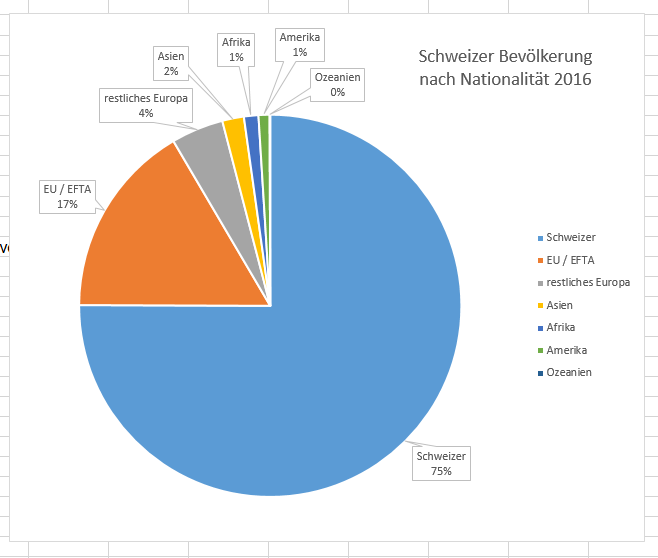
\includegraphics[width=0.7\linewidth]{GrundlagenInfo/09_Tabellenkalkulation/Screenshots/loesung-a}
\caption{Lösung zu a)}
\label{fig:loesung-a}
\end{figure}
\end{myanswer}
\begin{myanswer}
\begin{figure}[H]
\centering
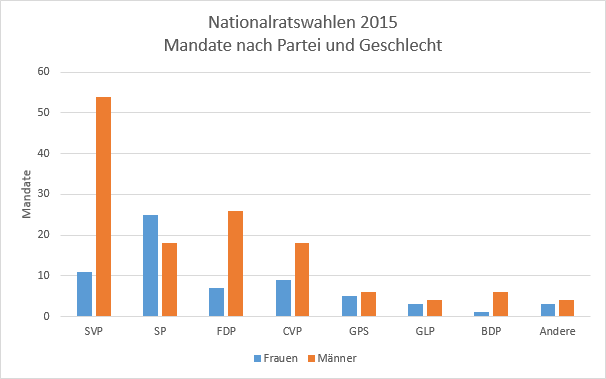
\includegraphics[width=0.7\linewidth]{GrundlagenInfo/09_Tabellenkalkulation/Screenshots/loesung-b}
\caption{Lösung zu b)}
\label{fig:loesung-b}
\end{figure}
\end{myanswer}
\begin{myanswer}
\begin{figure}[H]
\centering
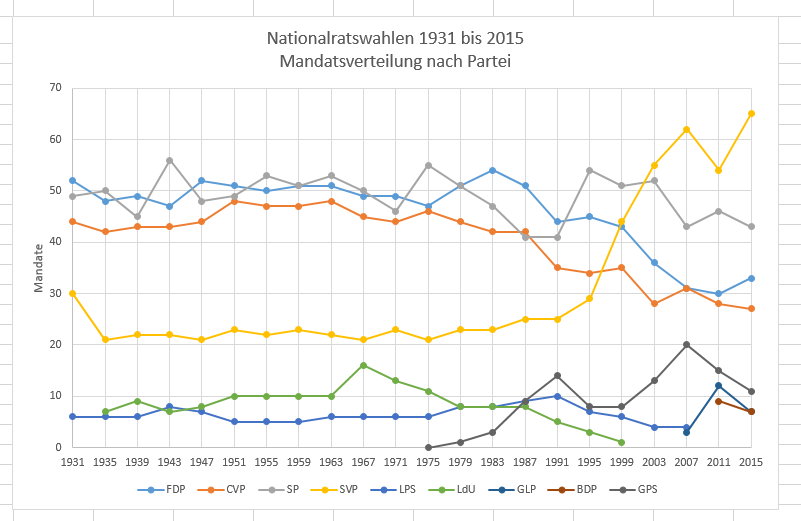
\includegraphics[width=0.7\linewidth]{GrundlagenInfo/09_Tabellenkalkulation/Screenshots/loesung-c}
\caption{Lösung zu c)}
\label{fig:loesung-c}
\end{figure}
\end{myanswer}
\begin{myanswer}
\begin{figure}[H]
\centering
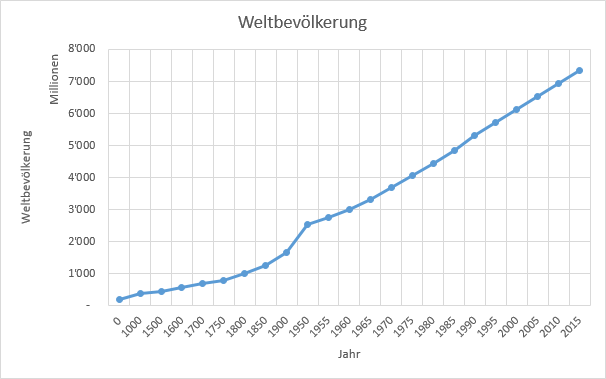
\includegraphics[width=0.7\linewidth]{GrundlagenInfo/09_Tabellenkalkulation/Screenshots/loesung-d-1}
\caption{Lösung zu d) (1)}
\label{fig:loesung-d-1}
\end{figure}
\end{myanswer}
\begin{myanswer}
\begin{figure}[H]
\centering
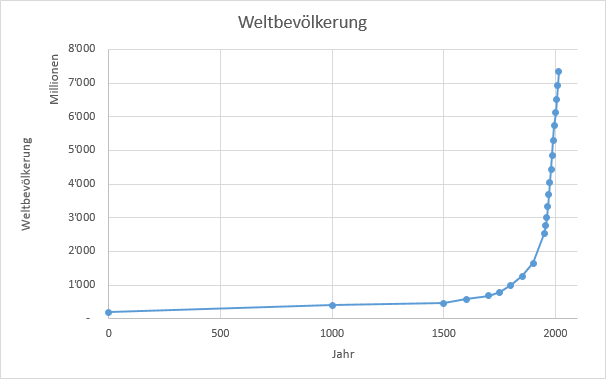
\includegraphics[width=0.7\linewidth]{GrundlagenInfo/09_Tabellenkalkulation/Screenshots/loesung-d-2}
\caption{Lösung zu d) (2)}
\label{fig:loesung-d-2}
\end{figure}
\end{myanswer}

\end{mysubmission}

\begin{mychallenge}
Normalerweise sind Daten für Diagramme nicht fertig aufbereitet verfügbar. Für die folgende Aufgabe müssen Sie die Daten selbst finden und in eine geeignete Tabelle überführen.

Erstellen Sie die folgenden Diagramme:
\begin{itemize}
\item Zeitliche Entwicklung der Maturitätsabschlüsse in der Schweiz, nach Geschlecht
\item Maturitätsabschlüsse in der Schweiz im Jahr 2016, Verteilung nach Schwerpunktfach
\end{itemize}
\textbf{Tipp}: Sie finden die nötigen Tabellen auf der Webseite des \href{https://www.bfs.admin.ch/bfs/de/home/statistiken.html}{Bundesamtes für Statistik}.

\end{mychallenge}

\begin{mychallenge}[Klimadiagramm]
Erstellen Sie ein Klimadiagramm für Bern mit den vorgegebenen Daten in der Arbeitsmappe \texttt{klima-bern}. Das Klimadiagramm soll so aussehen:
 
\begin{figure}[H]
\centering
\includegraphics[width=0.7\linewidth]{"GrundlagenInfo/09_Tabellenkalkulation/Screenshots/Klimadiagramm Bern"}
\label{fig:klimadiagramm-bern}
\end{figure}

Hinweise:
\begin{itemize}
\item Um ein kombiniertes Diagramm (Balken und Linien) zu erstellen, im Dialog ``Diagramm einfügen'' im Tab \texttt{Alle Diagramme} den Diagrammtyp \texttt{Verbund} auswählen.
\item Die Temperaturskala wird auf der Primärachse (links) dargestellt.
\item Die Niederschlagsskala wird auf der Sekundärachse (rechts) dargestellt.
\item Minimum und Maximum der beiden Skalen müssen so gewählt werden, dass die eine Skala ein Vielfaches der anderen Skala ist. Beispielsweise wird für die Temperatur eine Skala von -10 °C bis 60 °C gewählt und für den Niederschlag das Doppelte, also von -20 mm bis 120 mm.
\end{itemize}
\textbf{Wichtig}: Für das Klimadiagramm darf ausnahmsweise ein Liniendiagramm verwendet werden. Eigentlich wäre ein Punktdiagramm angebracht, aber da die Monatsnamen nicht Zahlen sind, kann dieses nicht eingesetzt werden.
Da alle Monate fast gleich lange sind, entsteht beim Liniendiagramm keine nennenswerte Verzerrung.

\end{mychallenge}

\begin{mysubmission}[Berechnungen (Sporttag)]
Speichern Sie die Arbeitsmappe \texttt{sporttag} auf Ihrem Computer.

\begin{itemize}
    \item Die Punktzahl beim Hochsprung ergibt sich aus der Höhe multipliziert mit dem angegebenen Faktor. Geben Sie in den Zellen der Spalte F Formeln ein, um die Punktzahl für jede/n Teilnehmer/in zu berechnen.
    \item Beim Weitsprung wird nur der beste Versuch berücksichtigt. Verwenden Sie in der Spalte K eine Funktion, um den besten Sprung für jede/n Teilnehmer/in zu bestimmen.
    \item Das Punktetotal ergibt sich, indem die Punkte aus Hochsprung und Weitsprung addiert werden. Fügen Sie in Spalte O entsprechende Formeln ein.
    \item Sortieren Sie die Tabelle nach dem Punktetotal absteigend.
    \item Schreiben Sie den Rang in die Spalte A.
\end{itemize}
Geben Sie einen Screenshot Ihrer fertigen Arbeitsmappe auf Moodle ab.
\end{mysubmission}

\begin{mysubmission}[Zellbezüge]
Verwenden Sie für diese Aufgabe die Arbeitsmappe \texttt{zellbezuege}.

\paragraph*{Telefontarif}
In der Zelle B3 ist der Minutentarif für Telefongespräche eingetragen.
\begin{itemize}
    \item Schreiben Sie in die Zelle B6 eine Formel, um den Preis zu berechnen.
    \item Verwenden Sie automatisches Ausfüllen, um die Formel in die Zellen B7 bis B12 zu kopieren.
    \item Geben Sie der Zelle B3 einen Namen und verwenden Sie diesen Namen in der Formel in Zelle B6.
    \item Verwenden Sie wieder automatisches Ausfüllen, um die Formel in die Zellen B7 bis B12 zu kopieren.
    \item Ändern Sie den Minutentarif. Was passiert?
\end{itemize}

\paragraph*{Währungen}
\begin{itemize}
    \item Geben Sie den Zellen B3 bis E3 einen Namen.
    \item Schreiben Sie in die Zelle B6 eine Formel, um den Preis zu berechnen.
    \item Verwenden Sie automatisches Ausfüllen, um die Formel in alle Zellen bis E12 zu kopieren. Was passiert?
\end{itemize}
Geben Sie einen Screenshot Ihrer fertigen Arbeitsmappe auf Moodle ab.
\end{mysubmission}

\begin{mysubmission}[Weizenkornlegende]
\paragraph*{Sissa ibn Dahir}
\begin{figure}[H]
\centering
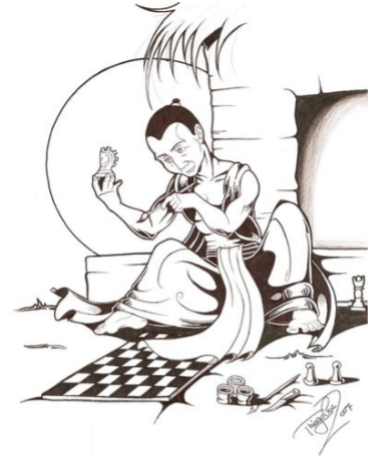
\includegraphics[width=0.3\linewidth]{GrundlagenInfo/09_Tabellenkalkulation/Screenshots/Sissa}
\end{figure}
Sissa ibn Dahir lebte angeblich im dritten oder vierten Jahrhundert in Indien und gilt Legenden zufolge als der Erfinder des Schachspiels.

\paragraph*{Weizenkornlegende}
Der indische Herrscher Shihram tyrannisierte seine Untertanen und stürzte sein Land in Not und Elend. Um die Aufmerksamkeit des Königs auf seine Fehler zu lenken, ohne seinen Zorn zu entfachen, schuf der weise Brahmane Sissa ein Spiel, in welchem der König als wichtigste Figur ohne Hilfe anderer Figuren und Bauern nichts ausrichten kann. Der Unterricht im Schachspiel machte auf den Herrscher Shihram einen starken Eindruck. Er wurde milder und ließ das Schachspiel verbreiten, damit alle davon Kenntnis nehmen.

Um sich für die anschauliche Lehre von Lebensweisheit und zugleich Unterhaltung zu bedanken, gewährte er dem Brahmanen einen freien Wunsch. Dieser wünschte sich Weizenkörner: Auf das erste Feld eines Schachbretts wollte er ein Korn, auf das zweite Feld das Doppelte, also zwei, auf das dritte wiederum die doppelte Menge, also vier und so weiter.

\paragraph*{Aufgabe A}
Sie sollen die Menge Weizenkörner, welche Sissa vom Herrscher gefordert hat, berechnen. Gehen Sie folgendermassen vor:
\begin{itemize}
    \item Erstellen Sie eine neue Arbeitsmappe im Tabellenkalkulationsprogramm.
    \item Schreiben Sie die Zahl Eins ins Feld A1.
    \item Schreiben Sie eine Formel ins Feld A2, welche die Zahl in A1 verdoppelt.
    \item Fahren Sie so weiter mit den Feldern A3 bis A8, dann B1 bis B8, usw.
\end{itemize}

\paragraph*{Aufgabe B}
Die Tausendkornmasse (Masse von 1’000 Körnern) von Weizen beträgt 40 bis 65 Gramm. 2016 betrug die weltweite Jahresproduktion von Weizen 749'460'078 Tonnen. Berechnen Sie im Tabellenkalkulationsprogramm, wie lange die ganze Welt auf Weizen verzichten müsste, um die Forderung von Sissa ibn Dahir zu erfüllen.

Geben Sie einen Screenshot Ihrer fertigen Arbeitsmappe auf Moodle ab.
\end{mysubmission}
\begin{mychallenge}
Formatieren Sie den Zellbereich A1:H8 wie ein Schachbrett:
\begin{itemize}
    \item Jedes zweite Feld hat einen schwarzen Hintergrund und eine weisse Schriftfarbe.
    \item Die Felder sind quadratisch.
\end{itemize}
\end{mychallenge}

\section*{Dank}
Spezieller Dank für diese Unterrichtsmaterialien geht an deren Ersteller Thomas Jampen und Martin Lehmann, Gymnasium Kirchenfeld Bern, \url{https://ict.mygymer.ch}

